\section{Durchführung}

    \subsection{Die Photozelle}
    Der in den theoretischen Grundlagen beschriebene Aufbau befindet sich in der Praxis in einem vakuumierten Glaskolben, dann Photozelle genannt.\\
    In der Photozelle wird die Photokathode allerdings so realisiert, dass auf der Innenseite des Kolbens eine Metallschicht aufgedampft wird.
    Die Anode ist dann ein dazu parallel verlaufender Draht, der sich in kleinem Abstand dazu befindet.\\
    Dieser Aufbau ist in Abbildung \ref{img:zelle} dargestellt.
    

    \begin{figure}[H]
        \centering
        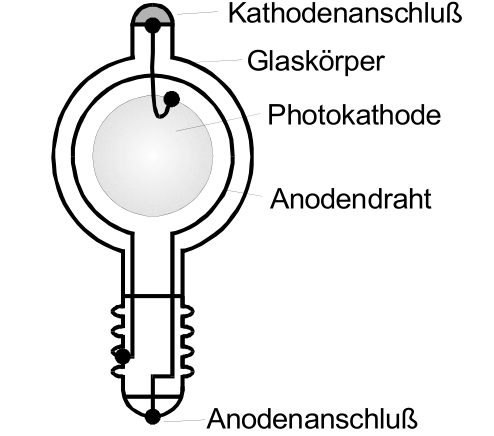
\includegraphics[width=0.35\textwidth]{latex/images/Photozelle.PNG}
        \caption{Der schematische Aufbau einer Photozelle wie sie in der Praxis verwendet wird\protect \cite{500}.}
        \label{img:schem}
    \end{figure}
    
    \begin{figure}[h]
        \centering
        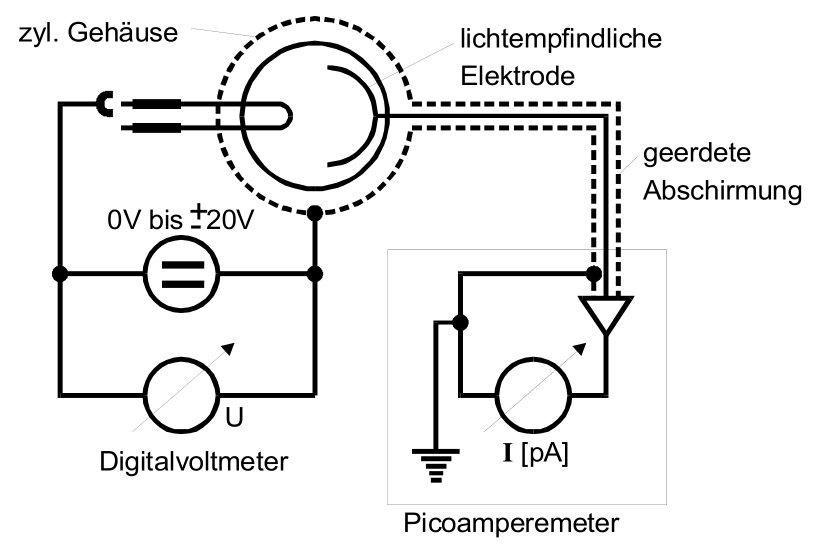
\includegraphics[width=0.5\textwidth]{latex/images/Schaltbild.PNG}
        \caption{Der schematische Aufbau einer Photozelle wie sie in der Praxis verwendet wird\protect \cite{500}.}
        \label{img:schem}
    \end{figure}

    \noindent Diese Zelle wird dann, wie in Abbildung \ref{img:Schaltbild}, geschaltet.
    Anders als in den Grundlagen beschrieben wird hier an die Photzelle ein entgegengesetztes Feld angelegt.
    Zur Untersuchung des Effektes wird hier mit der sogenannten Gegenfeldmethode gearbeitet.\\
    Die Elektronen werden weiterhin vom monochromatischen Licht herausgelöst müssen nun aber ein abbremsendes elektrisches Feld durchlaufen.
    Abhängig von der Anzahl der an der Anode gemessenen Elektronen und der angelegten Spannung lassen sich dann über die kinetische Energie 
    Rückschlüsse über die Geschwindkeitsverteilung der Elektronen schließen.\\
    Es können nun nämlich nur noch Elektronen die Anode erreichen deren kinetische Energie größer ist als $\symup{e} \cdot U$ mit $\symup{e}$ als Elementarladung\cite{e}.
    Der Strom versiegt also bei
    \begin{equation*}
        \symup{e} \cdot U= \frac{\symup{m_0}\cdot v_{max}}{2}
    \end{equation*}
    Wobei $\symup{m_0}$ die Ruhemasse des Elektrons \cite{massE} und $v_{max}$ die Geschwindigkeit der schnellsten Elektronen ist.\\
    Daraus folgt wiederum für diese Elektronen:
    \begin{equation}
        \symup{h}\cdot \nu= \symup{e} \cdot U + A_K
        \label{eqn:vmax}
    \end{equation}


    \subsection{Die Geschwindigkeitsverteilung}


    Der in Gleichung \ref{eqn:vmax} beschriebene Zusammenhang gilt aber nur für die schnellsten Elektronen.
    Dies sind die Elektronen, die schon in der Kathode die meiste kinetische Energie besitzen. 
    Dies führt dann für niedrigere Energien in der Kathode zu langsameren Elektronen.\\
    Dies ist auch in der folgenden Grafik veranschaulicht, welche dass mit steigender Bremsspannung kontinuierliche Abfallen der detektierten Photoelektronen zeigt.

    \begin{figure}[H]
        \centering
        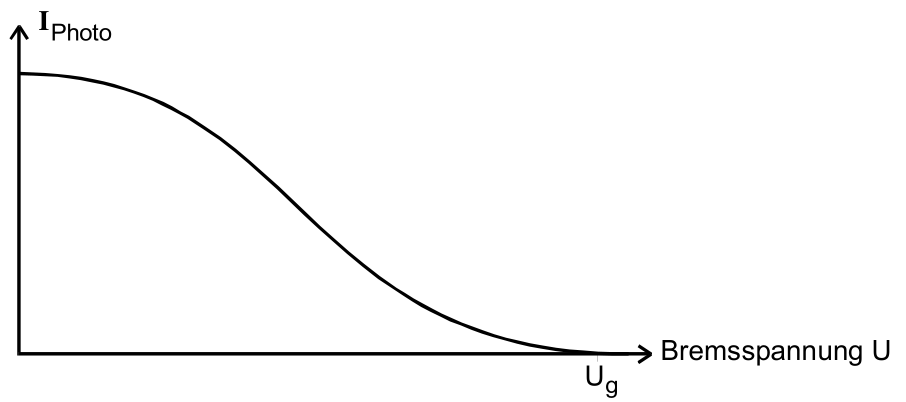
\includegraphics[width=0.7\textwidth]{latex/images/Bremsspannung.PNG}
        \caption{Ein Graph, welcher quantitativ das Abfallen des Photostroms mit steigender Bremsspannung zeigt \protect \cite{500}.}
        \label{img:brems}
    \end{figure}

    \noindent Die Energie der Elektronen in der Kathode lässt sich mit der Fermi-Dirac-Statistik beschreiben.\\
    Da diese aber hier nur begrenzt Gültigkeit besitzt, da nicht davon ausgegangen werden kann, dass alle Photoelektronen die flächenmässig kleine Anode erreichen.
    Deswegen lässt sich einfach die folgende, hier gültige, quadratische Abhängigkeit der des Photostroms von der Spannung nutzen:
    \begin{equation}
        I_{ph} \sim U^2
        \label{eqn:quad}
    \end{equation}

    Die Fermi-Niveaus $\zeta$ von Metallen, die in der Fermi-Dirac-Statistik beschrieben sind aber trotzdem noch für diesen Versuch relevant.\\
    Denn wenn zwei unterschiedliche Metalle aneinander angeschlossen werden gleichen sich ihre Fermi-Niveaus auf die gleiche Höhe an.\\
    Dies kann dazu führen, dass wenn die Austrittsarbeit der Anode $A_A$ größer ist als die Energie der Photonen, kein Photoeffekt auftritt, auch wenn die Energie größer ist als $A_K$.
    Um dann einen Photstrom zu messen muss ein beschleunigendes Potential $U_b$ angelegt werden, so dass gilt:
    \begin{equation*}
        \symup{h} \cdot \nu + \symup{e} \cdot U_b \geq A_A
    \end{equation*}
    Auf Grund dieses Effekts ässt sich sogar bei genügend großer Bremsspannung ein entgegengesetzten Photostrom messen, welcher Messungen beeinträchtigen kann.




    \subsection{Optischer Aufbau}

    Um zu gewährleisten, dass monochromatisches Licht genutzt wird, wird der in Abbildung \ref{img:linse} dargestellte Aufbau verwendet.


    \begin{figure}[H]
        \centering
        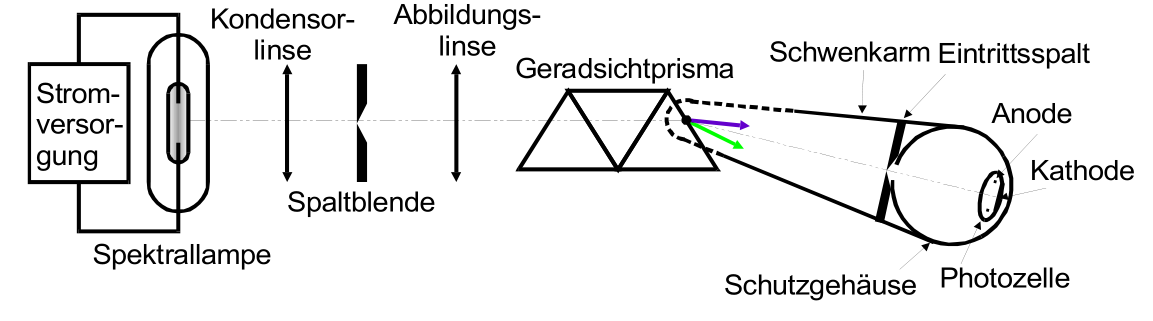
\includegraphics[width=0.7\textwidth]{latex/images/Optiken.PNG}
        \caption{Der optische Aufbau, welcher das Licht einer Spektrallampe aufspaltet  \protect \cite{500}.}
        \label{img:linse}
    \end{figure}

    Die Spektrallampe erzeugt hierbei Licht, welches von der Kondensorlinse gebündelt und durch die Spaltblende läuft.
    Anschließend wird das Licht wieder von der Abbildungslinse auf den Geradsichtprisma gebündelt, welcher das Licht in seine einzelnen Wellenlängen aufspaltet.
    Der Schwenkarm kann nun genutzt werden um die gewünschte Frequenz des Lichts auf die Photozelle strahlen zu lassen.\\
    Die wichtigsten Emissionslinien und Farben einer Quecksilberlampe sind in der folgenden Tabelle zu finden.

    \begin{figure}[H]
        \centering
        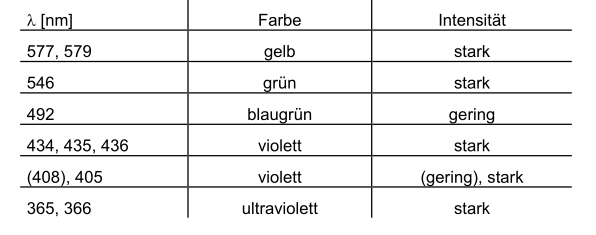
\includegraphics[width=0.6\textwidth]{latex/images/Hg.PNG}
        \caption{Die wichtigsten Linien einer Hg-Lampe\protect \cite{500}.}
        \label{img:Hg}
    \end{figure}